\documentclass[journal,compsoc]{IEEEtran}

% -- Encoding & Fonts ---------------------------------------------
\usepackage[T1]{fontenc}
\usepackage[utf8]{inputenc}

% -- Mathematics (light usage for magazine style) -----------------
\usepackage{amsmath,amssymb}

% -- Graphics & Figures -------------------------------------------
\usepackage{graphicx}

% -- Tables -------------------------------------------------------
\usepackage{booktabs}
\usepackage{array}

% -- Hyperlinks & References ---------------------------------------
\usepackage[hidelinks]{hyperref}
\usepackage{cite}
\usepackage{url}
\hypersetup{
  pdftitle={ARES: A Framework for Measuring Reliability and Failure Modes in Autonomous AI Security Agents},
  pdfauthor={Mohammad Makchudul Alam; Md. Redowan Z. Anik; Sabrein S. E. el Bodour; Moshiul Islam Mishu; Anca Delia Jurcut},
  pdfsubject={IEEE Security \& Privacy Magazine special issue on Autonomous AI Agents in Computer Security},
  pdfkeywords={ARES; AI security agents; reliability; SKC mismatch; Agent Reliability Score; Epistemic Gap; SOC; hallucination}
}

% -- Misc ---------------------------------------------------------
\usepackage{xcolor}
\usepackage{balance}
\usepackage{microtype}
\usepackage{enumitem}

% -- Framework name macros -----------------------------------------
\newcommand{\ARES}{\textsc{ARES}}
\newcommand{\ARESBench}{\textsc{ARES-Bench}}
\newcommand{\SAFK}{\textsc{SOCAgentFailure-1K}}

% -- TikZ styles ---------------------------------------------------

% -----------------------------------------------------------------
\begin{document}

\title{ARES: A Framework for Measuring Reliability and Failure Modes
in Autonomous AI Security Agents}

\author{%
\IEEEauthorblockN{%
Mohammad Makchudul Alam\textsuperscript{1,2},\,
Md.~Redowan Zaman Anik\textsuperscript{2},\,
Sabrein Serag El Din el Bodour\textsuperscript{2},\,
Moshiul Islam Mishu\textsuperscript{3},\,
and Anca Delia Jurcut\textsuperscript{4}%
\\[0.3em]
\textsuperscript{1}\textit{DNS Research Lab} \quad
\textsuperscript{2}\textit{BGD e-GOV CIRT, Dhaka, Bangladesh}\\
\textsuperscript{3}\textit{EIC Limited, Dhaka, Bangladesh} \quad
\textsuperscript{4}\textit{School of Computer Science, University College Dublin, Ireland}
}
}

\IEEEtitleabstractindextext{%
\begin{abstract}
% ===== sections/00_abstract =====
% 50-word abstract per IEEE S&P Magazine CFP requirement
Autonomous agents triage alerts in Security Operations Centres, yet
their failure conditions are poorly understood. \ARES{} models agent
failures as skill--knowledge--capability mismatches. Testing it against
600 live frontier-model executions reveals a calibration gap: agents
grow uncertain and abstain under knowledge deficit rather than
confidently hallucinate, inverting the assumed reliability risk.

\end{abstract}

\begin{IEEEkeywords}
AI agent reliability, cybersecurity, failure taxonomy, hallucination,
SOC automation, epistemic gap
\end{IEEEkeywords}
}

\maketitle

% ===== sections/01_introduction =====
\section{Introduction}

Security Operations Centres (SOCs) are undergoing a fundamental transformation.
Autonomous AI agents (powered by large language models (LLMs) and equipped
with tool-use capabilities) now perform threat detection, alert triage,
and incident response tasks that were previously the exclusive domain of
human analysts. Frameworks such as
LangGraph~\cite{langgraph2024} and AutoGen~\cite{wu2023autogen} have made it
straightforward to deploy multi-step reasoning agents that query SIEM systems,
correlate indicators of compromise (IOCs), and recommend containment actions
with minimal human oversight. Commercial platforms including CrowdStrike
Charlotte AI and SentinelOne Purple AI have begun embedding agent-based
automation into production SOC workflows, and the trend is accelerating.

Yet a critical question remains unanswered: \textit{when do these agents fail,
and how dangerous are those failures?} The security community has focused
heavily on measuring what AI agents can do (detection accuracy, response
speed, ATT\&CK coverage) while paying far less attention to the conditions
under which agents produce incorrect, incomplete, or actively misleading
outputs. This gap carries serious operational consequences:

\begin{itemize}[noitemsep, leftmargin=*]
  \item A \textbf{false negative} allows an intrusion to persist undetected
    for hours or days, expanding the attacker's foothold while the SOC
    believes the environment is clean.
  \item A \textbf{hallucinated threat attribution} propagates incorrect IOCs
    into shared intelligence feeds, poisoning downstream defences across
    multiple organisations that consume the same threat data.
  \item A \textbf{delayed response}, caused by an agent paralysed by missing
    tool access or overwhelmed by input complexity, allows an incident to
    escalate beyond regulatory reporting thresholds.
\end{itemize}

These are not hypothetical scenarios: they are predictable consequences of
deploying agents whose capabilities do not match the demands of their assigned
tasks. We call this the \textit{Skill--Knowledge--Capability (SKC) mismatch}
problem: the systematic gap between what a security task requires and what
an agent can actually deliver across multiple dimensions including procedural
skills, declarative threat knowledge, tool access, reasoning quality, and
knowledge currency.

Existing work addresses fragments of this problem in isolation. Classical
dependability theory~\cite{avizienis2004} predates LLM agents and has no
notion of epistemic uncertainty or knowledge currency.
Hallucination research~\cite{llmagent_halluc_survey2025} treats reasoning
failures as model-internal properties without modelling tool availability,
task complexity, or knowledge freshness. Calibration
work~\cite{guo2017calibration} shows neural networks are miscalibrated but
does not connect this to agent reliability. Agent
benchmarks~\cite{liu2023agentbench} measure capability
without modelling failure conditions. The closest
recent efforts, MAST~\cite{cemri2025mast}, a domain-agnostic 14-mode
failure taxonomy, and AgentDojo~\cite{debenedetti2024agentdojo}, an
adversarial prompt-injection environment, each cover one slice of
the surface. To the best of our knowledge, no existing work provides a
unified reliability model, evaluation testbed, and labelled failure
dataset for the full non-adversarial failure surface of AI security
agents.

\textbf{This paper presents \ARES{}} (Agentic Reliability Evaluation for
Security systems), a framework designed to fill this gap. \ARES{} provides:
\begin{enumerate}[noitemsep, leftmargin=*]
  \item A \textbf{three-axis failure taxonomy} classifying AI security agent
    failures by origin (8 classes), manifestation (8 classes), and operational
    impact (7 classes), grounded in CSIRT practice.
  \item A \textbf{quantitative reliability model} based on SKC mismatch,
    including an Agent Reliability Score (ARS) with task-class-specific
    weights and an Epistemic Gap metric that formalises the hallucination
    precondition.
  \item \textbf{\ARESBench{}}, a fully open-source, Docker-deployable
    evaluation testbed supporting four agent architectures across five
    threat scenario classes.
  \item \textbf{\SAFK{}}, an analytical corpus of 1,000 agent execution
    traces under controlled failure conditions, released under CC~BY~4.0.
  \item A \textbf{calibration-gap finding}: testing the model's central
    assumption against 600 live frontier-agent executions, we show that
    real agents grow uncertain and abstain under knowledge deficit
    rather than confidently hallucinate, inverting the risk the failure
    model, and much of the literature, assumes.
\end{enumerate}

Together they let SOC architects screen an agent for a given task before
it sees production traffic, and, as importantly, tell them which of the
model's assumptions survive contact with real agents.

Parallel 2025--2026 efforts confirm the urgency: hallucination
benchmarks~\cite{bang2025hallulens} treat confident factual errors as
a cross-domain failure class, and the OWASP Top~10 for Agentic
Applications~\cite{owasp2026agentic} elevates capability-mismatch and
tool-misuse failures to first-class operational risks. None of these
efforts connect agent reliability to SOC-specific consequences: a
misclassified ransomware beacon or a fabricated CVE attribution.
\ARES{} fills that gap.

% ===== sections/02_why_reliability =====
\section{Why Reliability of AI Agents Matters for Cybersecurity}

The reliability of AI agents is not merely an academic concern: it is an
operational safety requirement. When an AI agent operates autonomously in a
SOC, its outputs directly influence incident response decisions that affect
the security posture of entire organisations. Unlike traditional software,
where bugs produce deterministic incorrect outputs, LLM-based agents
introduce a qualitatively different failure surface: \textit{stochastic,
context-dependent, and confidence-inflated errors} that are difficult to
detect and dangerous to act upon.

\textbf{Risks of autonomous AI decisions.}
A human analyst who encounters an unfamiliar threat pattern will typically
escalate or seek additional context. An LLM-based agent, by contrast, may
confidently classify a novel threat using superficially similar patterns from
its training data, a failure mode known as hallucination. In cybersecurity,
hallucination is particularly dangerous because the domain is dense with
specific factual claims (CVE identifiers, threat actor names, TTP chains)
that are easy to fabricate convincingly but difficult to verify in
real time~\cite{llmagent_halluc_survey2025}. The consequences of
incorrect autonomous decisions are often irreversible: once a compromised
host is left un-isolated or a fabricated IOC enters a shared feed, the damage
propagates faster than human review can contain it.

\textbf{Impact on incident response.}
Consider a three-stage pipeline: triage, enrichment, and remediation.
If triage misclassifies a ransomware intrusion as a benign false
positive, enrichment never investigates and remediation recommends no
action, so the intrusion persists and exfiltration proceeds undetected.
If instead triage hallucinates a threat-actor attribution, for example
pinning a commodity phishing campaign on an APT group, enrichment may
propagate fabricated IOCs to shared STIX/TAXII feeds, corrupting
defences across every organisation that consumes them. A third agent
lacking EDR containment access (capability mismatch) may identify the
threat correctly yet fail to execute isolation, introducing a critical
response delay.

\textbf{Trust and accountability.}
SOC analysts must trust agent outputs enough to act on them, but not so
much that they stop verifying. Agents that fail silently, plausible but
wrong, erode that calibration: repeated false confidence pushes analysts
into either over-reliance (automation complacency) or disengagement
(automation aversion), both degrading effectiveness. Under regulatory
frameworks such as NIS2 or DORA the challenge compounds, since
incident-response decisions must be traceable whether a human or an agent
made the call.

\textbf{Why hallucination is uniquely dangerous in SOC environments.}
Hallucination in security operations is \textit{actionable}. A hallucinated
medical diagnosis triggers further tests; a hallucinated legal citation is
caught in review; but a hallucinated threat attribution can trigger immediate
containment (host isolation, feed updates) with real cost and often no
verification checkpoint before execution. High confidence, factual density,
and automated downstream actions make SOC hallucination uniquely dangerous
among AI application domains.

\textbf{Why existing assurance approaches fall short.}
Classical software testing does not catch stochastic, context-dependent
agent failures: a test suite that passes at build time says nothing about
reliability under a new CVE or novel ransomware variant. SOC peer review
is the safety net for sensitive decisions, but autonomous agents are
deployed precisely to remove that bottleneck. Adversarial ML benchmarks
measure robustness against crafted perturbations rather than against the
benign-but-unfamiliar inputs that dominate SOC workload. Hallucination
benchmarks~\cite{bang2025hallulens} count how often models fabricate
facts but do not connect fabrication to the downstream security actions
that turn a wrong answer into operational harm. These gaps motivate a
structured framework for measuring agent reliability \textit{before
deployment} and monitoring it \textit{during operation}, which is what
\ARES{} provides.

% ===== sections/03_failure_taxonomy =====
\section{Failure Taxonomy for AI Security Agents}

Understanding \textit{how} agents fail is a prerequisite for measuring
reliability. We propose a three-axis taxonomy that decomposes each
failure event along three orthogonal dimensions: what caused it
(\textit{origin}), what it looked like (\textit{manifestation}), and
what it cost (\textit{impact}). Unlike prior fault taxonomies developed
for conventional software~\cite{avizienis2004}, this taxonomy is
designed specifically for autonomous AI security agents, where
failures are not bugs to be patched but operational risks that affect
real-world security outcomes. Table~\ref{tab:taxonomy_mag} summarises
the three axes.

\begin{table}[t]
\caption{Three-Axis Failure Taxonomy for AI Security Agents}
\label{tab:taxonomy_mag}
\centering
\footnotesize
\setlength{\tabcolsep}{3pt}
\begin{tabular}{p{0.85cm} p{2.5cm} p{4.0cm}}
\toprule
\textbf{Code} & \textbf{Class} & \textbf{Description} \\
\midrule
\multicolumn{3}{l}{\textit{Axis 1: Origin (root cause)}} \\
O1 & Epistemic Deficiency & Lacks required threat knowledge \\
O2 & Skill Boundary & Task requires an unlearned procedure \\
O3 & Capability Deprivation & Required tool or API unavailable \\
O4 & Reasoning Corruption & Inference produces invalid output \\
O5 & Context Overload & Input exceeds processing capacity \\
O6 & Adversarial Perturbation & Malicious content degrades output \\
O7 & Orchestration Failure & Multi-agent coordination breakdown \\
O8 & Temporal Drift & Knowledge has become stale \\
\midrule
\multicolumn{3}{l}{\textit{Axis 2: Manifestation (observable signal)}} \\
M1 & Hallucination & Asserts verifiably false facts \\
M2 & Omission & Fails to detect a present threat \\
M3 & Misclassification & Wrong threat family or category \\
M4 & Confabulation & Coherent reasoning from false premises \\
M5 & Paralysis & No output or persistent retry loop \\
M6 & Overclaiming & High confidence on weak evidence \\
M7 & Attribution Error & Wrong threat actor or campaign \\
M8 & Cascade Failure & Error propagates across agents \\
\midrule
\multicolumn{3}{l}{\textit{Axis 3: Impact (operational consequence)}} \\
I1 & False Negative\hfill\textbf{*} & Threat undetected; attacker persists \\
I2 & False Positive & Benign activity flagged \\
I3 & Delayed Response & Action issued past SLA \\
I4 & Wrong Remediation\hfill\textbf{*} & Incorrect containment executed \\
I5 & Intelligence Pollution\hfill\textbf{*} & Fabricated IOCs propagate to feeds \\
I6 & Trust Erosion & Analyst confidence reduced \\
I7 & Compliance Violation & Regulatory threshold breached \\
\bottomrule
\multicolumn{3}{l}{\footnotesize \textbf{*}\;Critical impact category.} \\
\end{tabular}
\end{table}

Two distinctions matter for practitioners. First, \textit{Hallucination}
(M1) and \textit{Confabulation} (M4) are not synonyms. Hallucination
asserts atomic facts that are verifiably false against a closed-world
corpus; confabulation produces internally coherent reasoning founded
on non-existent premises. Confabulation is more dangerous because it
is harder to detect by automated checks and more persuasive to
analysts reviewing the agent's reasoning trace. Second,
\textit{Intelligence Pollution} (I5) is qualitatively unlike the other
impacts: a single hallucinated IOC pushed to a STIX/TAXII feed
propagates beyond the originating organisation to the entire
information-sharing community.

The power of the three-axis decomposition is its diagnostic
composability. A practitioner who observes a cluster of M1 events can
trace back to O1 (knowledge deficiency) or O5 (context overload) as
the most probable origins, and forward to I1 (false negative) or I5
(intelligence pollution) as the likely consequences. Each origin maps
to a distinct operational action: O1 calls for knowledge refresh, O5
for input preprocessing, O3 for tool provisioning.

\textbf{Worked example: Intelligence Pollution.}
A pipeline correctly identifies a phishing campaign, but the enrichment
stage invents three IOC URLs by extrapolating a domain pattern; a
downstream automation pushes them to the shared feed, and within minutes
partner SOCs block legitimate subdomains of a real service. The trace
decomposes cleanly: origin O1 (missing TTP chain), manifestation M1
(hallucinated facts), impact I5 (blast radius beyond the originating
organisation), and it motivates per-IOC confidence gating,
confidence-proportional feed propagation, and human review for feed
writes, each traceable to a distinct axis.

% ===== sections/04_reliability_model =====
\section{Reliability Model: SKC Mismatch}

The taxonomy tells us \textit{how} agents fail; the reliability model tells
us \textit{why} and \textit{how likely}. At its core, \ARES{} measures the
gap between what a security task demands and what an agent can deliver across
five dimensions. The model extends classical dependability
theory~\cite{avizienis2004} by introducing knowledge incompleteness,
probabilistic reasoning errors, and capability constraints as first-class
failure sources: dimensions that do not exist in traditional deterministic
software systems.
Figure~\ref{fig:skc_pipeline_mag} summarises the end-to-end flow.

\begin{figure}[t]
\centering
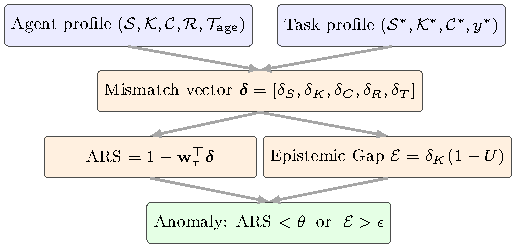
\includegraphics{fig1_skc_pipeline.pdf}
\caption{The \ARES{} reliability pipeline. The agent's declared
profile and the task's requirement profile produce a five-dimensional
mismatch vector that feeds two parallel indicators: the Agent
Reliability Score and the Epistemic Gap. Either crossing its learned
threshold flags the execution as anomalous.}
\label{fig:skc_pipeline_mag}
\end{figure}

\subsection{Five Mismatch Dimensions}

For each dimension, we compute a normalised mismatch score between 0 (full
coverage) and 1 (total mismatch); we summarise each here and specify how it
is measured on a real agent in Section~\ref{sec:aresbench}. Full formal definitions of the
agent and task profiles and of each indicator (as set-cardinality ratios
over the task's required skills, ATT\&CK TTP subgraph, and tool manifest,
with an exponential-decay temporal term) are given in the companion
technical paper~\cite{alam2026ares}.

\begin{itemize}[noitemsep, leftmargin=*]
  \item \textbf{Skill mismatch} ($\delta_S$): the fraction of required
    procedural skills the agent lacks. For example, a log-correlation agent
    assigned binary malware analysis has a high $\delta_S$ because the
    required analytical procedure is outside its repertoire.
  \item \textbf{Knowledge mismatch} ($\delta_K$): the fraction of required
    threat knowledge missing from the agent's context, measured over the
    MITRE ATT\&CK~\cite{strom2022} knowledge graph. An agent unaware of a
    recently emerged ransomware variant has high $\delta_K$ for tasks
    involving that family.
  \item \textbf{Capability mismatch} ($\delta_C$): the fraction of
    required tools or APIs the agent cannot access. An agent that recommends
    host isolation but lacks EDR API access has high $\delta_C$: it knows
    \textit{what} to do but cannot \textit{do} it.
  \item \textbf{Reasoning mismatch} ($\delta_R$): the divergence between
    the agent's output and ground truth, capturing inference quality. This
    dimension is unique in that it can only be measured post-execution.
  \item \textbf{Temporal drift} ($\delta_T$): knowledge staleness modelled
    as exponential decay, parameterised by the threat domain's volatility.
    Ransomware intelligence ($\lambda = 0.005$~day$^{-1}$) decays rapidly;
    APT attribution knowledge ($\lambda = 0.001$~day$^{-1}$) remains stable
    for longer.
\end{itemize}

A critical design property: the first three dimensions ($\delta_S$,
$\delta_K$, $\delta_C$) and temporal drift ($\delta_T$) can all be computed
\textit{before} task execution from the agent's declared profile and the
task's requirements. In deployment, \ARES{} therefore uses skill,
knowledge, capability, and temporal drift for pre-execution
screening; reasoning mismatch ($\delta_R$) is used after execution
for diagnosis and model improvement.

\subsection{Agent Reliability Score}

The five mismatch scores are combined into a single
\textbf{Agent Reliability Score (ARS)}:
\[
  \mathrm{ARS} = 1 - \mathbf{w}_\tau^\top \boldsymbol{\delta}
\]
where $\boldsymbol{\delta} = [\delta_S, \delta_K, \delta_C, \delta_R,
\delta_T]$ is the mismatch vector and $\mathbf{w}_\tau$ is a weight vector
specific to the threat class $\tau$, learned via ridge regression on labelled
training data. An ARS of 1.0 indicates perfect alignment between agent
capability and task demand; values below a learned threshold $\theta^*$
flag the agent as unreliable for that task.

The weights are learned per threat class because different security tasks
stress different dimensions. On the analytical corpus, knowledge coverage
($w_K = 0.35$) dominates for ransomware detection, skill and capability
access ($w_S = 0.32$, $w_C = 0.28$) lead for DDoS mitigation, and knowledge
with reasoning ($w_K = 0.38$, $w_R = 0.24$) lead for APT investigation;
within that model a universal weight vector misestimates reliability by at
least 12\% on some classes. These values illustrate the model's structure
and must be re-fit on a deployer's own labelled outcomes.

\subsection{Epistemic Gap: The ``Confident Ignorance'' Problem}

The most dangerous agent failures occur not when an agent lacks knowledge,
but when it \textit{does not know that it lacks knowledge}, a failure of
confidence calibration~\cite{guo2017calibration}. We formalise this as the
\textbf{Epistemic Gap}:
\[
  \mathcal{E} = \delta_K \times (1 - U)
\]
where $U$ is the agent's expressed uncertainty (complement of its stated
confidence). An agent with a large knowledge deficit ($\delta_K \approx 1$)
that simultaneously reports high confidence ($U \approx 0$) produces a
maximal Epistemic Gap: the precondition for hallucination. Conversely, an
agent that correctly identifies its knowledge limits ($U \approx 1$) produces
a near-zero Epistemic Gap: it may fail the task but will not fabricate
an answer. Whether the dangerous regime actually arises is an empirical
question, and one much of the hallucination literature answers by
assumption. We test it directly (Empirical Insights) and find that real
frontier agents keep $U$ high as $\delta_K$ rises, so the maximal-gap
precondition is the exception rather than the rule, which makes
$\mathcal{E}$ valuable precisely as a detector of that exception.

This concept relates directly to the confidence calibration literature, which
has shown that modern neural networks (including LLMs) are systematically
overconfident on out-of-distribution inputs~\cite{guo2017calibration}. The
Epistemic Gap operationalises this finding for the specific case of agentic
AI: it measures not just whether the model is miscalibrated in general, but
whether that miscalibration occurs precisely where the agent's knowledge is
weakest: the most dangerous combination.

The distinction is critical for SOC operations. An agent that says
``I don't have sufficient context to classify this threat'' is safe: it
triggers human escalation. An agent that confidently asserts a false threat
attribution is dangerous: it triggers automated actions based on fabricated
intelligence.

\subsection{Cascade Reliability in Multi-Agent Systems}

When agents are composed into pipelines, failures propagate through
information dependencies. We model this using a directed acyclic graph
where each edge represents an inter-agent data flow, and show that cascade
reliability is bounded above by the \textit{weakest agent} in the pipeline.

This result has a counterintuitive practical consequence: decomposing
a security task into a multi-agent pipeline cannot improve reliability
beyond the weakest component agent. It can only reduce it. A triage agent
that hallucinates an IOC passes corrupted input downstream, where
enrichment inherits and amplifies it and the recommendation agent acts
on the compounded error. Our analytical results decompose this effect
cleanly. Under a matched-bucket ablation on the analytical corpus
(reported in the Empirical Insights section),
the reliability loss is attributable almost entirely to pipeline depth
rather than to the choice of agent framework, and is roughly three
times the size the naive headline gap between single-agent and
three-stage pipelines would suggest.

\subsection{From Score to Action}

Operationally, an ARS assessment runs at task-assignment time and
yields three control points. If ARS clears the threshold, the agent
runs autonomously. If it falls short, the decomposition itself
identifies the cheapest mitigation: a high $\delta_K$ calls for a
knowledge refresh, a high $\delta_C$ for tool provisioning, and a
high $\delta_T$ for a scheduled retraining cadence. The Epistemic
Gap is computed at output time and gates downstream propagation:
high-$\mathcal{E}$ outputs go to human review rather than to
automated containment or shared threat feeds. Because four of the
five dimensions are observable before execution, the screening cost
is effectively zero.

% ===== sections/05_ares_bench =====
\section{\ARESBench{} Evaluation Framework}
\label{sec:aresbench}

To validate the reliability model empirically, we built
\ARESBench{}: an open-source, Docker-deployable testbed for measuring
AI security agent reliability under controlled conditions. The design
prioritises reproducibility (single-command deployment, all data
sources public and versioned), generalisability (multiple agent
architectures and threat classes), and controllability (systematic
mismatch injection across a structured matrix). The full architecture
diagram, data-source manifest, and measurement-pipeline details are
maintained in the project artefact repository (see Section~\ref{sec:conclusion}).

\textbf{Agents under test.} \ARESBench{} evaluates four agent
architectures spanning the major paradigms: \textbf{AUT-1
(LangGraph)}~\cite{langgraph2024}, a stateful graph-based ReAct loop;
\textbf{AUT-2 (AutoGen)}~\cite{wu2023autogen}, a three-stage
multi-agent pipeline (triage $\to$ enrichment $\to$ recommendation);
\textbf{AUT-3 (CrewAI)}, a role-based crew (analyst, enrichment,
incident commander); and \textbf{AUT-4}, a deterministic Sigma/YARA
evaluator with no LLM component, serving as the $\delta_R = 0$
control. Hallucination is structurally impossible in AUT-4. In live mode the
testbed drives these agents with a local Mistral-7B-Instruct backbone
via Ollama; the released \SAFK{} corpus, however, uses the analytical
path (below), and the live calibration and cascade studies use hosted
frontier models, not Ollama.

\textbf{Controlled mismatch injection.} A Mismatch Injector applies
controlled degradation across four dimensions ($\delta_S, \delta_K,
\delta_C, \delta_R$) at four levels each (0, 0.33, 0.66, 1.0).
Mechanisms are deliberately realistic: disabling tool nodes in the
agent's execution graph ($\delta_S$); filtering ATT\&CK TTP context
from retrieval to retain only a controlled fraction ($\delta_K$);
intercepting API calls via a middleware proxy that returns
permission-denied errors ($\delta_C$); and inserting misleading content
into the system prompt at controlled probability ($\delta_R$).
Temporal drift ($\delta_T$) is set parametrically via the agent's
knowledge-age attribute.

\textbf{Failure measurement.} An Anomaly Monitor parses agent
output, cross-references claims against ATT\&CK and NVD as a
closed-world ground truth, and flags any unverifiable claim asserted
with confidence $> 0.70$ as a hallucination candidate. It then
computes the five mismatch dimensions, the ARS, and the Epistemic Gap,
and assigns taxonomy labels using a rule-based engine validated
against human annotations (Cohen's $\kappa = 0.84$ for origin,
$\kappa = 0.91$ for manifestation).

\textbf{From injection to measurement.} Controlled injection is how we
\textit{construct} the study, not how the model is instantiated in
deployment: each dimension is computed from artefacts a SOC already
possesses. \textit{Skill} ($\delta_S$) and \textit{capability}
($\delta_C$) are read from the agent's registered tool and function
manifest, the fraction of the task's required procedures and APIs it is
not wired to invoke. \textit{Knowledge} ($\delta_K$) is measured over
context, not weights: the fraction of the task kill-chain's ATT\&CK TTP
nodes absent from the agent's retrieval index or supplied context,
exactly computable for a retrieval-augmented agent; a genuinely novel
threat matches nothing and drives $\delta_K \to 1$, precisely the
high-risk regime the score should flag. \textit{Temporal drift}
($\delta_T$) uses time since the last knowledge refresh, and expressed
uncertainty $U$ is the agent's stated confidence. Four of the five
dimensions are thus prospective, needing no run-time ground truth; only
$\delta_R$ requires post-hoc comparison. The live-incident harness
(Empirical Insights) exercises this path on real CVEs, with no
injection.

\textbf{The \SAFK{} corpus (analytical).} \SAFK{} is a labelled corpus
of 1{,}000 traces stratified across five threat classes (200 each),
four agent architectures (250 each), and 16 mismatch conditions.
Crucially, its \textit{outcomes}, hallucination, expressed confidence,
task success, and the taxonomy labels, are generated from the mismatch
inputs by closed-form models, not read from live execution. This makes \SAFK{} an analytical instrument: mismatch--failure
relationships can be studied under exact ground truth and reproduced
deterministically, at the cost of encoding rather than discovering
them, which is why this article's central claim is validated not on
\SAFK{} but on live agents. The corpus is released under CC BY 4.0
alongside the code.

\textbf{The live-agent harness.} To test the model's assumptions
against reality, \ARESBench{} also drives \textit{real} agents: it
applies the same $\delta_K$ manipulation to the prompt of a
frontier LLM, then measures hallucination against ATT\&CK ground truth
and records the agent's own expressed confidence. This is the path
behind the calibration-gap result and the live-incident study
(Empirical Insights); the harness and its 600-execution output are
released with the corpus so the comparison is reproducible. Because
frontier models are stochastic and served behind evolving endpoints,
re-running the harness reproduces the reported \textit{effects}
(rising uncertainty and flat fabrication under increasing $\delta_K$)
directionally rather than the exact per-call values; the committed
run log is the frozen record behind every number we report.

% ===== sections/06_empirical_insights =====
\section{Empirical Insights}

We first report the result that most changed our own view of the
problem, then the analytical findings that motivated the test. The
headline is a \textit{calibration gap}: the reliability model, like the
broader literature it builds on, assumes that knowledge deficit drives
\textit{confident} fabrication, but real frontier agents do the
opposite, they express uncertainty and abstain. Practitioners should
therefore calibrate their expectations to real model behaviour, not to
the failure model.

\subsection{The Calibration Gap: Real Agents Abstain Where the Model
Predicts Hallucination}

\textbf{Setup.} \SAFK{} is an \textit{analytical} corpus: its outcomes
(hallucination, confidence, task success) are generated from the
mismatch inputs by calibrated closed-form models, so that the
mismatch--failure relationships can be studied under known ground
truth. That construction encodes a specific assumption drawn from the
hallucination literature, that an agent's expressed confidence stays
high as its knowledge degrades (``confident ignorance''), producing a
steep $\delta_K \to$ hallucination dose-response. We tested that
assumption directly against live agents.

We ran \textbf{600 real executions} across five frontier backbones
spanning two model families (Claude Haiku~4.5, Sonnet~4.6, and
Opus~4.7; GPT-4o-mini and GPT-4o) on ten ATT\&CK-grounded SOC
scenarios. Knowledge mismatch $\delta_K$ was applied as a genuine
manipulation, withholding a controlled fraction of the scenario's
ground-truth TTP context from the prompt, and every outcome was
\textit{measured} from real output: the agent either named a primary
ATT\&CK technique (correct, or a fabrication if absent from ground
truth) or abstained (``insufficient information''), together with its
stated confidence.

\textbf{Finding.} The assumed dose-response does not hold
(Table~\ref{tab:calib_mag}). Where the analytical model rises to a
39\% fabrication rate at $\delta_K = 1$ with correlation $\rho = 0.92$,
real fabrication stays low (0--20\%) and only weakly related to $\delta_K$
(pooled Pearson $\rho = 0.11$; at most $0.27$ for any single model). The mechanism is calibration: real
confidence \textit{falls} as knowledge is withheld (Pearson $\rho$
between $-0.35$ and $-0.51$ across all five models, both families),
inverting the built-in overconfidence the failure model assumes.
Because expressed uncertainty rises exactly when knowledge drops, the
``confident ignorance'' precondition rarely materialises, and confident
fabrication, the dangerous quadrant the whole framework targets, occurs
in at most 13\% of executions. The effect scales with capability: the
most capable model, Claude Opus~4.7, fabricated in \textbf{0\%} of 120
executions and instead raised its abstention rate from 10\% at
$\delta_K = 0$ to 67\% at $\delta_K = 1$, while the smallest,
GPT-4o-mini, is the least calibrated (13\% confident fabrication) yet
still far short of the model's 39\%. That the same pattern holds across
two independent model families is the point: it is not a quirk of one
vendor's alignment but a general property of current frontier agents.

\begin{table}[t]
\caption{Calibration gap: analytical failure model vs.\ 600 live agent
executions across two model families. The top row is the failure model's
\emph{assumed} behaviour; all agent rows are \emph{measured}. Fabrication is
scored against ATT\&CK ground truth; confidence is the agent's stated value.}
\label{tab:calib_mag}
\centering
\footnotesize
\setlength{\tabcolsep}{3.5pt}
\begin{tabular}{lcccc}
\toprule
 & $\rho(\delta_K,$ & fab.\ at & $\rho(\delta_K,$ & conf.\ \\
\textbf{Agent} & fab.$)$ & $\delta_K{=}1$ & conf.$)$ & risk \\
\midrule
\SAFK{} \emph{(assumed)} & $+0.92$ & 0.39 & $\approx 0$ & high \\
\midrule
Haiku 4.5          & $+0.05$ & 0.13 & $-0.45$ & 0.09 \\
Sonnet 4.6         & $+0.27$ & 0.17 & $-0.35$ & 0.07 \\
Opus 4.7           & $\approx 0$ & \textbf{0.00} & $-0.40$ & \textbf{0.00} \\
GPT-4o-mini        & $+0.07$ & 0.20 & $-0.50$ & 0.13 \\
GPT-4o             & $+0.17$ & 0.07 & $-0.51$ & 0.03 \\
\bottomrule
\multicolumn{5}{l}{\footnotesize ``conf.\ risk'' = rate of confident
fabrication (wrong \& conf.\ $\geq 0.7$).}
\end{tabular}
\end{table}

This corroborates our second real-data probe. On 30 live CISA KEV
incidents disclosed after every model's training cutoff (so $\delta_K
\approx 1$ by construction), five frontier LLMs scored identically on
surface accuracy (vendor 67\%, product 63\%, CVE $\leq$3\%), yet
confidence behaviour diverged: the OpenAI models answered almost
every record at mean confidence 0.68--0.78, whereas the strongest
Claude model abstained on 26 of 30 rather than assert an unsupported
attribution.\footnote{The specific models evaluated are named above; their
exact API version strings and evaluation dates for all runs are recorded in
the artefact repository so every result is reproducible.} Both
studies point the same way: whether an agent hallucinates under
knowledge deficit is not a property of the deficit but of the model's
calibration, and modern frontier models are calibrated to abstain.

\textbf{Comparison to calibration baselines.} By the standard metric the
agents are well-calibrated: pooled expected calibration error
(ECE)~\cite{guo2017calibration} is $0.04$ (Brier $0.09$; $n=419$ answered
runs), well below the levels reported for uncalibrated deep networks. This
is exactly why raw verbalized confidence~\cite{tian2023calibration} alone
barely predicts fabrication (AUROC
$0.51$, chance level): a calibrated agent is confident on both correct
answers and the rare miss. The Epistemic Gap, which fires only when high
$\delta_K$ meets high confidence, separates fabrication better than either
single-signal baseline (AUROC $0.68$, versus $0.62$ for $\delta_K$ and
$0.51$ for confidence), and confidence-ordered selective
prediction~\cite{elyaniv2010selective} cuts
error from $10\%$ at full coverage to $1\%$ at $25\%$ coverage.

\textbf{Implication.} Do not assume that missing threat knowledge
translates into confident fabrication; on well-calibrated agents it
translates into \textit{abstention and reduced coverage}. The
first-order deployment risk shifts accordingly, from ``the agent will
confidently invent a threat attribution'' to ``the agent will decline
to act, and a poorly-calibrated agent in the fleet is the exception
that still fabricates.'' Reliability tooling should therefore watch the
confidence signal, not the knowledge gap alone, and treat a
low-abstention, high-confidence agent as the anomaly.

\subsection{Different Mismatches Produce Distinct Failure Signatures}

\textbf{Finding (analytical).} Within \SAFK{}, each mismatch dimension
maps to a diagnostically separable manifestation (chi-square test of
independence, $p < 0.001$): capability deprivation ($\delta_C$)
predominantly produces \textit{Paralysis} (78\%); skill deficit
($\delta_S$) produces silent \textit{Omission} (72\%); knowledge gaps
($\delta_K$) produce \textit{Hallucination} (32\%) and
\textit{Misclassification} (21\%); reasoning perturbation ($\delta_R$)
produces \textit{Confabulation} (38\%) and \textit{Overclaiming}
(17\%). Because these mappings are built into the model, we present them
as the taxonomy's \textit{design}, a hypothesis about how root causes
surface, not an independent empirical discovery.

\textbf{Implication.} The manifestation pattern is a diagnostic
fingerprint a SOC can validate on its own telemetry: high paralysis points
at tool/API access rather than LLM quality; high confabulation at reasoning
corruption or adversarial input rather than knowledge gaps.

\subsection{The Epistemic Gap Targets the Residual Risk}

\textbf{Finding.} The calibration gap does not make hallucination
harmless, it relocates it. Confident fabrication still occurs, just in
a minority of executions (0--13\% above) concentrated in weaker or
mis-prompted agents. This is precisely the case the \textbf{Epistemic
Gap} $\mathcal{E} = \delta_K \times (1 - U)$ is built to isolate: it is
large only when knowledge is low \textit{and} expressed confidence is
high. On well-calibrated agents, rising $\delta_K$ is met by rising
uncertainty, so $\mathcal{E}$ stays small and the gate correctly stays
quiet; on the residual confident-ignorance cases, $\mathcal{E}$ spikes.
The metric's value is thus not a headline correlation but a factoring
of risk into a ``what the agent does not know'' term ($\delta_K$) and a
``how confidently it acts under that ignorance'' term ($1 - U$), of
which our data show the \textit{second} to be the operative one.

\textbf{Implication.} Calibration is the actionable lever. Because
real agents already hedge under ignorance, the highest-value
intervention is to preserve and monitor that hedging, gate high-$\mathcal{E}$
outputs to human review, and flag any agent whose confidence fails to
fall as its knowledge does.

\subsection{Multi-Agent Composition: Bound and Live Test}

\textbf{Finding (analytical).} Within the model, composing agents into
a pipeline cannot raise reliability above the weakest stage. A
matched-bucket ablation on \SAFK{} attributes the AUT-1 vs.\ AUT-2 gap
almost entirely to pipeline depth (17.25\%) rather than framework
identity (0.13\%), and the analytic weakest-link bound holds in 100\%
of the 250 pipeline records (zero violations).

\textbf{Live test.} Running the same attribution task as a single agent
versus a tightly-coupled three-stage pipeline (three models, 120 paired
trials, temperature 0.7, identical token budget; only depth varies)
confirms the bound's \emph{direction} but not its magnitude: end-to-end
reliability drops from $0.86$ to $0.82$, a small but significant
$3.3$~pp degradation (95\% CI $[0.8, 6.7]$), and pipeline reliability
never exceeds the single agent in any cell. The penalty is
model-dependent, not universal ($7.5$, $2.5$ and $0.0$~pp for
Haiku~4.5, Sonnet~4.6 and GPT-4o-mini; two of three per-model intervals
include zero). As with the calibration gap, the
analytical model over-states the live failure rate: real pipelines
degrade far less than its encoded $17\%$ depth effect.

\textbf{Implication.} Treat multi-agent decomposition as a reliability
cost to justify, not a default: prefer validated single-agent designs
for critical tasks, and if composition is required, add inter-stage
verification and confidence-gated propagation so a low-confidence
intermediate does not silently seed downstream stages.

% ===== sections/07_implications =====
\section{Deployment Guidance for SOC Teams}

\ARES{} translates into concrete guidance for teams deploying
autonomous AI agents, organised around six questions SOC architects
face when integrating agentic AI, and closing with a five-step
pre-deployment checklist.

\textbf{When should AI agents be trusted?}
ARS is proposed as a pre-execution screening signal: an agent scoring
below a learned threshold is escalated to a human or reconfigured
(add knowledge context, restore tool access). The threshold is
deployment-specific and must be fit on the deployer's own labelled
outcomes, not transplanted (our analytical corpus is illustrative
only). Because four of the five dimensions ($\delta_S, \delta_K,
\delta_C, \delta_T$) are computable before execution, screening adds no
runtime overhead and slots into SOAR platforms as a pre-condition for
autonomous execution~\cite{nist_ai_rmf}. ARS is a screening heuristic,
not a validated detector; the calibration signal below is the
empirically supported lever.

\textbf{How can reliability be monitored continuously?}
The Epistemic Gap enables runtime hallucination risk monitoring: by
comparing the agent's stated confidence against its known knowledge
coverage, a monitor flags high-risk outputs for human review before
they trigger automated actions, valuable for host isolation, threat
feed updates, and evidence preservation. Computing $\mathcal{E}$
requires only the agent's confidence and pre-computed $\delta_K$,
both already in the execution record.

\textbf{How should knowledge maintenance be scheduled?}
The temporal-drift model gives the \textit{shape} of a per-domain
update schedule: reliability decays at a domain-specific rate
$\lambda$, so fast-moving domains need more frequent refresh.
Illustrative constants ($\lambda = 0.005$~day$^{-1}$ for ransomware,
$0.001$ for APT attribution) imply roughly quarterly versus annual
refresh, but must be fit on each deployer's own drift data; the
contribution is the schedule form, not these numbers.

\textbf{How should multi-agent systems be designed?}
Composition never beat the best single agent live, but the penalty was
small ($3.3$~pp) and model-dependent, not the large amplification the
model predicts. Treat decomposition as a reliability cost to justify,
not a default: measure the depth penalty for your own backbone. Where
composition is warranted, three mitigations reduce cascade risk: (1)
inter-agent verification checkpoints; (2) confidence-gated propagation
(low-confidence outputs go to humans, not downstream); (3) redundant
agent paths for critical decisions.

\textbf{How can safer agent systems be built?}
Our calibration-gap result reorders the usual priorities. (1)
\textit{Calibration-first design}, the operative lever: prefer and
validate agents whose expressed confidence falls as their knowledge
degrades, since it is calibration, not knowledge coverage alone, that
determines whether a knowledge gap becomes a confident fabrication.
(2) \textit{Knowledge coverage} still matters, but chiefly for
\textit{task success}: a well-calibrated but under-informed agent will
abstain safely, trading coverage for reliability, so knowledge refresh
is a capability investment more than a safety one. (3) \textit{Fail-safe
defaults}, preserve and reward the abstention behaviour real agents
already exhibit, rather than prompting them to always answer. The one
agent configured or fine-tuned to answer confidently under uncertainty
is the dangerous exception, and the one to screen out.

\textbf{How does this map to regulatory and governance frameworks?}
The NIST AI Risk Management
Framework~\cite{nist_ai_rmf} identifies ``valid and reliable,''
``accountable and transparent,'' and ``safe'' as top-tier
trustworthiness characteristics: \ARES{} operationalises the first
via ARS, the second via the traceable mismatch decomposition, and
the third via the Epistemic-Gap escalation gate. At the application layer,
the OWASP Top~10 for Agentic
Applications~\cite{owasp2026agentic} catalogues capability
over-provisioning, tool misuse, and confident hallucination as
distinct risk categories, each of which has a direct analogue in
\ARES{}: $\delta_C$ over-provisioning, $\delta_C$ plus $\delta_R$
tool misuse, and the Epistemic Gap for confident hallucination.

\textbf{A deployment checklist.}
Distilling the above into a pragmatic checklist for SOC
architects yields five steps: \textit{(i)} estimate pre-execution
$\delta_S$, $\delta_K$, $\delta_C$, $\delta_T$ for each intended
task class; \textit{(ii)} apply the task-class-specific weight
vector and compare ARS against a threshold fit on local labelled
outcomes; \textit{(iii)}
if ARS is below threshold, choose one of three mitigations
(knowledge refresh, capability provisioning, or task-scope
restriction) and re-score; \textit{(iv)} instrument the runtime
to emit stated confidence alongside each decision and compute
$\mathcal{E}$ per record, and prefer agents whose confidence
falls under withheld knowledge; \textit{(v)} schedule knowledge
refreshes according to a domain-specific temporal-drift
constant fit on local drift data. Each step maps to a concrete
engineering artefact, so the reliability gate does not stay
theoretical.

% ===== sections/08_limitations =====
\section{Limitations and Future Work}

\textbf{Analytical corpus.} \SAFK{}'s outcomes are generated from the
mismatch inputs by closed-form models, so its dose-response, taxonomy
signatures, and cascade bound \textit{encode} the relationships they
describe rather than discover them. We treat them as an organising
model, and it is exactly this that the calibration-gap experiment tests:
the model's central assumption (confident ignorance under knowledge
deficit) did not survive contact with real agents. The taxonomy
manifestation mapping has not yet been re-measured on live agents and
should be read as a hypothesis; the cascade bound's \emph{direction} is
confirmed live (a small $3.3$~pp degradation, Empirical Insights), but its magnitude at
greater pipeline depths and scales remains open.

\textbf{Scale and scope of the live study.} The calibration-gap result
rests on 600 executions across five backbones spanning the Claude and GPT families, ten
ATT\&CK-grounded scenarios, and a single-technique attribution task,
complemented by 30 post-cutoff CISA KEV incidents across five models.
This is enough to overturn a universal claim, that frontier agents
confidently hallucinate under knowledge deficit as a rule, but not to
characterise the full distribution of agent behaviour: fabrication is
low (0--20\%) and flat in $\delta_K$ rather than absent. Broader model
coverage (including open-weight and non-frontier agents, where
calibration is weaker), more scenarios, multi-step tool-using agents,
and larger real-incident corpora are the natural next steps.

\textbf{Closed-world hallucination labels.} Fabrication is scored
against ATT\&CK/NVD as ground truth, so a genuinely-related technique
absent from a scenario's curated set can be counted as a fabrication;
this makes our real fabrication rates, already low, if anything an
over-estimate, which strengthens rather than weakens the calibration-gap
conclusion.

\textbf{Confidence as expressed, not verified.} We use the agent's
self-reported confidence. This is the operative signal a monitor would
actually read, but eliciting well-calibrated confidence remains an open
problem; a poorly-calibrated agent that reports high confidence under
ignorance is exactly the residual risk the Epistemic Gap is meant to
catch.

Future work re-measures the taxonomy signatures on live agents, extends
the cascade test to deeper pipelines and the calibration study across
agent architectures, and connects the confidence signal to runtime
gating in a production SOC.

% ===== sections/09_conclusion =====
\section{Conclusion}
\label{sec:conclusion}

As AI agents take on greater operational responsibility in defending
critical infrastructure, frameworks for understanding their failure
behaviour become a prerequisite for responsible deployment. \ARES{}
contributes an integrated treatment for the cybersecurity domain: a
three-axis failure taxonomy, a skill--knowledge--capability reliability
model with an Agent Reliability Score and an Epistemic Gap metric, an
open testbed, and an analytical corpus for reproducible study. To be
explicit about scope: what this article \emph{validates} on real agents
is the calibration gap and the Epistemic Gap as a fabrication-risk
detector; the taxonomy, the ARS weights, and the cascade magnitude are
analytical structure to be re-fit and re-measured per deployment, not
empirical rates.

Our central result, however, is a corrective one. The reliability
model, in common with much of the hallucination literature, assumes
that knowledge deficit produces \textit{confident} fabrication. Tested
against 600 live frontier-agent executions and a post-cutoff live-CVE
study, that assumption inverts: real agents are calibrated, their
expressed confidence falls as their knowledge degrades, so they abstain
rather than confidently hallucinate, and confident fabrication, the
failure the framework is built to catch, occurs in a small minority of
cases concentrated in the least-calibrated agents. Knowledge coverage
is therefore not the first-order reliability lever the model implies;
\textit{calibration} is.

The practical guidance follows: monitor the confidence signal, not the
knowledge gap alone; gate high-Epistemic-Gap outputs; and treat a
low-abstention, high-confidence agent under uncertainty as the anomaly.
More broadly, the result is a caution for the field: reliability claims
about autonomous agents should be validated on real agents, because the
failure modes a plausible model predicts are not always the ones that
occur.

\ARES{}, \ARESBench{}, \SAFK{}, and the live calibration dataset are
publicly released to support reproducible research in AI security agent
dependability.\footnote{\url{https://github.com/IntelEyes/ARES-Framework}}


% Generated by IEEEtran.bst, version: 1.14 (2015/08/26)
\begin{thebibliography}{10}
\providecommand{\url}[1]{#1}
\csname url@samestyle\endcsname
\providecommand{\newblock}{\relax}
\providecommand{\bibinfo}[2]{#2}
\providecommand{\BIBentrySTDinterwordspacing}{\spaceskip=0pt\relax}
\providecommand{\BIBentryALTinterwordstretchfactor}{4}
\providecommand{\BIBentryALTinterwordspacing}{\spaceskip=\fontdimen2\font plus
\BIBentryALTinterwordstretchfactor\fontdimen3\font minus
  \fontdimen4\font\relax}
\providecommand{\BIBforeignlanguage}[2]{{%
\expandafter\ifx\csname l@#1\endcsname\relax
\typeout{** WARNING: IEEEtran.bst: No hyphenation pattern has been}%
\typeout{** loaded for the language `#1'. Using the pattern for}%
\typeout{** the default language instead.}%
\else
\language=\csname l@#1\endcsname
\fi
#2}}
\providecommand{\BIBdecl}{\relax}
\BIBdecl

\bibitem{langgraph2024}
{LangChain Inc.}, ``{LangGraph}: Building stateful, multi-actor applications
  with {LLMs},'' \url{https://github.com/langchain-ai/langgraph}, 2024,
  accessed: March 2025.

\bibitem{wu2023autogen}
Q.~Wu, G.~Bansal, J.~Zhang, Y.~Wu \emph{et~al.}, ``{AutoGen}: Enabling next-gen
  {LLM} applications via multi-agent conversation,'' 2023.

\bibitem{avizienis2004}
A.~Avizienis, J.-C. Laprie, B.~Randell, and C.~Landwehr, ``Basic concepts and
  taxonomy of dependable and secure computing,'' \emph{IEEE Transactions on
  Dependable and Secure Computing}, vol.~1, no.~1, pp. 11--33, 2004.

\bibitem{llmagent_halluc_survey2025}
X.~Lin, Y.~Ning, J.~Zhang, Y.~Dong \emph{et~al.}, ``{LLM}-based agents suffer
  from hallucinations: A survey of taxonomy, methods, and directions,''
  \emph{arXiv preprint arXiv:2509.18970}, 2025.

\bibitem{guo2017calibration}
C.~Guo, G.~Pleiss, Y.~Sun, and K.~Q. Weinberger, ``On calibration of modern
  neural networks,'' in \emph{Proceedings of the 34th International Conference
  on Machine Learning (ICML)}, 2017, pp. 1321--1330.

\bibitem{liu2023agentbench}
X.~Liu, H.~Yu, H.~Zhang, Y.~Xu \emph{et~al.}, ``{AgentBench}: Evaluating {LLMs}
  as agents,'' in \emph{Proceedings of the International Conference on Learning
  Representations (ICLR)}, 2024.

\bibitem{cemri2025mast}
M.~Cemri, M.~Z. Pan, S.~Yang, L.~A. Agrawal, B.~Chopra, R.~Tiwari, K.~Keutzer,
  A.~Parameswaran, D.~Klein, and K.~Ramchandran, ``Why do multi-agent {LLM}
  systems fail?'' in \emph{Advances in Neural Information Processing Systems
  ({NeurIPS})}, 2025.

\bibitem{debenedetti2024agentdojo}
E.~Debenedetti, J.~Zhang, M.~Balunovi{\'c}, L.~Beurer-Kellner, M.~Fischer, and
  F.~Tram{\`e}r, ``{AgentDojo}: A dynamic environment to evaluate prompt
  injection attacks and defenses for {LLM} agents,'' in \emph{Advances in
  Neural Information Processing Systems ({NeurIPS})}, 2024.

\bibitem{bang2025hallulens}
Y.~Bang, D.~Chen, N.~Lee, and P.~Fung, ``{HalluLens}: {LLM} hallucination
  benchmark,'' in \emph{Proceedings of the 63rd Annual Meeting of the
  Association for Computational Linguistics ({ACL})}, 2025.

\bibitem{owasp2026agentic}
{OWASP Foundation}, ``{OWASP} top 10 for agentic applications (2026),''
  \url{https://genai.owasp.org/resource/owasp-top-10-for-agentic-applications-for-2026/},
  2026, accessed: April 2026.

\bibitem{alam2026ares}
M.~M. Alam, M.~R.~Z. Anik, S.~S.~E. el~Bodour, and A.~D. Jurcut, ``{ARES}: A
  formal reliability framework for detecting anomalous behaviour in agentic
  {AI} systems,'' in \emph{Proc.\ IEEE Int.\ Conf.\ on Intelligent Systems and
  Interdisciplinary Applications (ISAIA)}, Montclair, NJ, USA, Oct. 2026.

\bibitem{strom2022}
B.~E. Strom, A.~Applebaum, D.~P. Miller \emph{et~al.}, ``{MITRE ATT\&CK}:
  Design and philosophy,''
  \url{https://attack.mitre.org/docs/ATTACK_Design_and_Philosophy_March_2020.pdf},
  2020.

\bibitem{tian2023calibration}
K.~Tian, E.~Mitchell, A.~Zhou, A.~Sharma, R.~Rafailov, H.~Yao, C.~Finn, and
  C.~D. Manning, ``Just ask for calibration: Strategies for eliciting
  calibrated confidence scores from language models fine-tuned with human
  feedback,'' in \emph{Proceedings of the 2023 Conference on Empirical Methods
  in Natural Language Processing ({EMNLP})}, 2023.

\bibitem{elyaniv2010selective}
R.~El-Yaniv and Y.~Wiener, ``On the foundations of noise-free selective
  classification,'' \emph{Journal of Machine Learning Research}, vol.~11, pp.
  1605--1641, 2010.

\bibitem{nist_ai_rmf}
{National Institute of Standards and Technology}, ``Artificial intelligence
  risk management framework ({AI RMF} 1.0),'' National Institute of Standards
  and Technology, Tech. Rep. AI 100-1, 2023.

\end{thebibliography}

\balance

% -- Author biographies --------------------------------------------
% Override IEEEtran's bio environment with a tight magazine-style
% format so all five bios fit on the same page.
\renewenvironment{IEEEbiographynophoto}[1]{%
  \par\vspace{0.35em}%
  \noindent\textbf{#1}\space\ignorespaces}{%
  \par}
\begin{IEEEbiographynophoto}{Mohammad Makchudul Alam}
is a Researcher with the DNS Research Lab specialising in agentic
AI reliability and failure characterisation in autonomous security
operations.
\end{IEEEbiographynophoto}

\begin{IEEEbiographynophoto}{Md.~Redowan Zaman Anik}
is an Incident Handler with BGD e-GOV CIRT, focusing on SOC
automation and AI-assisted incident response.
\end{IEEEbiographynophoto}

\begin{IEEEbiographynophoto}{Sabrein Serag El Din el Bodour}
is a System Analyst with BGD e-GOV CIRT, contributing scenario
grounding and failure-trace labelling to \ARES{}.
\end{IEEEbiographynophoto}

\begin{IEEEbiographynophoto}{Moshiul Islam Mishu}
is a PCI-DSS Auditor and Cybersecurity Professional with EIC Limited,
Dhaka, Bangladesh, specialising in PCI-DSS audits, VAPT, SOC, and GRC.
\end{IEEEbiographynophoto}

\begin{IEEEbiographynophoto}{Anca Delia Jurcut}
is an Assistant Professor at University College Dublin specialising
in network security, anomaly detection, and trustworthy AI for
cybersecurity.
\end{IEEEbiographynophoto}

\end{document}
